\chapter{Wybrane zagadnienia propagacji fal w ośrodku sprężystym - Bartłomiej Piwowarczyk}
\label{cha:wybrane_zagadnienia_propagacji_fal_w_osrodku_sprezystym}

W rozdziale przedstawiono zagadnienia dotyczące mechaniki ośrodka sprężystego wykorzystywane w projekcie. Założenia liniowej teorii sprężystości oraz definicje naprężenia i odkształcenia przytaczane są w \cite{bartek_wolny}. Opis typów fal sprężystych znaleźć można w \cite{bartek_rose} i \cite{bartek_nazarchuk}. Zjawisko dyspersji opisane jest między innymi w \cite{bartek_rose}, \cite{bartek_feruza}, \cite{bartek_cervena}, \cite{bartek_tian}, \cite{bartek_valsamos}, a sposoby wyznaczania krzywych wzbudzalności w \cite{bartek_kijanka} oraz \cite{bartek_fabien}. Efekt sing-around jest obiektem prac \cite{bartek_kwach} oraz \cite{bartek_kwach2}. Przetworniki piezoeletryczne były analizowane na podstawie danych dostępnych na stronie jednego z producentów \cite{bartek_piezo}.


%---------------------------------------------------------------------------



\section{Liniowa teoria sprężystości}
\label{sec:liniowa_teoria_sprezystosci}

Liniowa teoria sprężystości jest mechaniką ciała stałego opartą na następujących założeniach:
\begin{itemize}
  \item ciało jest wypełnione materią w sposób ciągły zarówno przed jak i po odkształceniu
  \item odkształcenia i przemieszczenia są bardzo małe
  \item spełniona jest zasada superpozycji
  \item ośrodek zachowuje się zgodnie z prawem Hooke'a
  \item siły działają na ciało w taki sam sposób przed odkształeceniem jak i po odkształceniu
\end{itemize}

\subsection{Naprężenie}
\label{sec:naprezenie}

Naprężenie można zdefiniować jako miara sił wewnętrznych ciała w punkcie. Weźmy ciało przedstawione na rysunku \ref{fig:potato}, na które działają siły zewnętrzne P1 i P2. W płaszczyźnie przekroju wybieramy punkt B, w którego otoczeniu określamy pole dA. Stosunek sił jakimi oddziałują na siebie połówki ciała w tym punkcie przekroju, do pola dA, nazywamy naprężeniem ciała w punkcie B. Kierunek naprężenia będzie zgodny z kierunkiem działania siły przekrojowej w punkcie.

\begin{figure}[h]
\centering
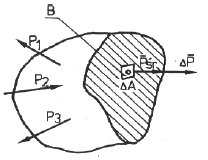
\includegraphics[width=5cm]{Zdjecia/2/potato}
\caption{Ciało pod wpływem sił zewnętrznych \cite{bartek_wolny}}
\label{fig:potato}
\end{figure}

Stana naprężenia w punkcie B oznacza ogół naprężeń, które otrzymamy dla wszystkich możliwych przekrojów ciała przez ten punkt.
W przypadku trójwymiarowego stanu naprężenia, dla każdego przekroju wektor naprężenia będzie miał inny kierunek. Stan naprężenia można opisać przy pomocy tensora naprężeń, dla układu kartezjańskiego danego wzorem:


\begin{gather}
	\sigma=\begin{bmatrix} 
	  \sigma_{xx}    & \tau_{xy} & \tau_{xz} \\ 
	  \tau_{yx} & \sigma_{yy} & \tau_{yz} \\
	  \tau_{zx} & \tau_{zy} & \sigma_{zz} 
	\end{bmatrix}
\end{gather}

gdzie

\begin{eqwhere}[2cm]
        \item[$\sigma_{ii}$] naprężenie normalne, i=(x, y, z)
        \item[$\tau_{ij}$] naprężenie styczne, i,j=(x, y, z), \( i \neq j, \tau_{ij}=\tau_{ji}\)
\end{eqwhere}

\subsection{Odkształcenie i prawko Hooke'a}
\label{sec:odksztalcenie_i_prawo_hookea}

	Pod wpływem naprężeń ciało sprężyste ulega odkształceniu. Możemy wyróżnić odkształcenia liniowe \( \varepsilon_i \) oraz odkształcenia postaciowe \( \gamma_{ij} \). Najprostszym przypadkiem odkształcenia liniowego jest rozciąganie pręta. Poniżej znajduje się rysunek pręta rozciąganego siłą P. 

\begin{figure}[h]
\centering
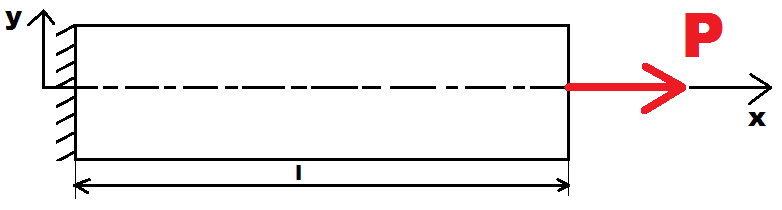
\includegraphics[width=10cm]{Zdjecia/2/rozciaganie}
\caption{Rozciąganie pręta}
\label{fig:rozciaganie}
\end{figure}

	W takim przypadku odkształceniem wzdłużnym będziemy nazywać stosunek wydłużenia pręta do jego początkowej długości:

\begin{equation}
\varepsilon_x=\frac{\Delta l}{l}.
\end{equation}
	
	Odkształceniem poprzecznym(postaciowym) nazywać będziemy stosunek zmiany średnicy przekroju do jego początkowej średnicy:

\begin{equation}
\varepsilon_y=\frac{\Delta d}{d}.
\end{equation}

	Odkształcenia te związane są zależnością:

\begin{equation}
\varepsilon_x=-\nu \varepsilon_y
\end{equation}
gdzie
\begin{eqwhere}[2cm]
        \item[$\nu$] współczynnik Poissona.
\end{eqwhere}

	Współczynnik Poissona jest wielkością bezwymiarową. Określa on sposób w jaki odkształca się ciało i przyjmuje wartości z przedziału [-1, 1]. Dla popularnych w mechanice stopów metali przyjmuje zwykle wartości z przedziału [0.2 , 0.4]. Wartości ujemne przyjmuje dla tak zwanych materiałów odwrotnych, które pod wpływem naprężenia zwiększają swoją objętość.

	Dla przypadku prostego rozciągania zachodzi jeszcze jedna zależność. Opisuje ona związek pomiędzy naprężeniem i odkształceniem i nazywana jest prawem Hooke'a.

\begin{equation}
\sigma=E\varepsilon
\end{equation}
gdzie
\begin{eqwhere}[2cm]
        \item[$E$] moduł Younga.
\end{eqwhere}

	Moduł Younga określa zależność odkształcenia liniowego i przyłożonego naprężenia. Jednostką moduły Younga jest paskal, a wartości podaje się w gigapasklach (GPa). Wartości dla stali wynoszą około 200 GPa, a dla aluminium około 70 GPa.

	W przypadku trójwymiarowego rozkładu okształceń stosuje się zapis tensorowy. Tensor odkształcenia znajduje się poniżej:
\begin{gather}
	\varepsilon=\begin{bmatrix} 
	  \varepsilon_{xx}    & \gamma_{xy} & \gamma_{xz} \\ 
	  \gamma_{yx} & \varepsilon_{yy} & \gamma_{yz} \\
	  \gamma_{zx} & \gamma_{zy} & \varepsilon_{zz} 
	\end{bmatrix}
\end{gather}

%\[
%	\textbf{$\varepsilon$}=\begin{bmatrix} 
%	  \varepsilon_{xx}    & \gamma_{xy} & \gamma_{xz} \\ 
%	  \gamma_{yx} & \varepsilon_{yy} & \gamma_{yz} \\
%	  \gamma_{zx} & \gamma_{zy} & \varepsilon_{zz} 
%	\end{bmatrix}
%\]

gdzie

\begin{eqwhere}[2cm]
        \item[$\varepsilon_{ii}$] odkształcenie liniowe, i=(x, y, z)
        \item[$\gamma_{ij}$] odkształcenie postaciowe, i,j=(x, y, z), \( i \neq j, \tau_{ij}=\tau_{ji}\)
\end{eqwhere}

Dla takiego przypadku prawo Hooke'a przybiera bardziej skomplikowaną postać:

\begin{equation}
\varepsilon_xx=\frac{1}{E}(\sigma_xx-\nu(\sigma_yy+\sigma_zz)), \gamma_{xy}=\frac{\tau_{xy}}{G}
\end{equation}
\begin{equation}
\varepsilon_yy=\frac{1}{E}(\sigma_yy-\nu(\sigma_xx+\sigma_zz)), \gamma_{xz}=\frac{\tau_{xz}}{G}
\end{equation}
\begin{equation}
\varepsilon_zz=\frac{1}{E}(\sigma_zz-\nu(\sigma_xx+\sigma_yy)), \gamma_{yz}=\frac{\tau_{yz}}{G}
\end{equation}

\begin{eqwhere}[2cm]
        \item[$G$] moduł Kirchoffa
\end{eqwhere}

	Moduł Kirchoffa opisuje zależność odkształcenia postaciowego od naprężenia stycznego występującego w materiale. Jednostką tego współczynnika jest paskal, a typowymi wartościami są dla stali 80 Gpa, dla aluminium 25,5 GPa.

	Opisane wcześniej stałe materiałowe są powiązane równaniem:
\begin{equation}
E=2G(\nu+1)
\end{equation}

%\begin{equation}
%c_L=\sqrt{\frac{\lambda+2\mu}{\rho}}
%\end{equation}
%gdzie
%\begin{eqwhere}[2cm]
%        \item[$c_L$] prędkość fali podłużnej
%        \item[$\lambda, \mu$] stałe Lam\'{e}go
%        \item[$\rho$] gęstość ośrodka
%\end{eqwhere}
%
%\begin{figure}[h]
%\centering
%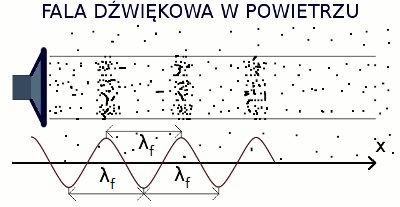
\includegraphics[width=10cm]{Zdjecia/2/fala_podluzna}
%\caption{Przykład fali podłużnej}
%\label{fig:fala_podluzna}
%\end{figure}
%
%
%
%\begin{figure}[h]
%        \centering
%        \begin{subfigure}{0.35\textwidth}
%                \centering
%	     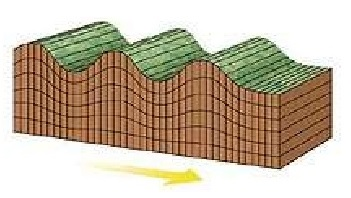
\includegraphics[width=5cm]{Zdjecia/2/fala_rayleigha}
%                \subcaption{\label{subfigure_a}}
%        \end{subfigure}
%        \begin{subfigure}{0.35\textwidth}
%                \centering
%	     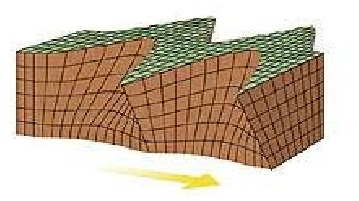
\includegraphics[width=5cm]{Zdjecia/2/fala_lova}
%                \subcaption{\label{subfigure_b}}
%        \end{subfigure}
%        \label{fig:subcaption_example}
%        \caption{Fale powierzchniowe: \protect\subref{subfigure_a} fala Rayleigha, \protect\subref{subfigure_b} fala L\"{o}va}
%\end{figure}

























\section{Rodzaje fal sprężystych}
\label{sec:rodzaje_fal_sprezystych}

Fale można podzielić ze względu na sposób w jaki propagują w materiale. Mogą to być fale podłużne lub poprzeczne. Fale takie propagują jeśli długość fali jest mniejsza lub bliska wymiarom ośrodka. Fale o długości przekraczającej wyraźnie przynajmniej jeden z wymiarów falowodu nazywamy falami prowadzonymi i mają one zupełnie inne własności. Do takich fal możemy zaliczyć np. fale Lamba. Fala Rayleigha z kolei propagują na powierzchniach, stąd ośrodek musi być ograniczony przynajmniej jedną płaszczyzną.

\subsection{Fale podłużne}

Fale podłużne to fale, w których kierunek propagacji jest równoległy z kierunkiem drgania cząstek. Tego typu fale mogą rozchodzić się w każdym ośrodku materialnym. Przykładem fali podłużnej jest fala dźwiękowa rozchodząca się w powietrzu, pokazana na Rys.2.1. Prędkoś fali podłużnej w nieograniczonym ośrodku zależy od parametrów materiałowych ośrodka i dana jest wzorem:

\begin{equation}
c_L=\sqrt{\frac{\lambda+2\mu}{\rho}}
\end{equation}
gdzie
\begin{eqwhere}[2cm]
        \item[$c_L$] prędkość fali podłużnej
        \item[$\lambda, \mu$] stałe Lam\'{e}go
        \item[$\rho$] gęstość ośrodka
\end{eqwhere}

\begin{figure}[h]
\centering
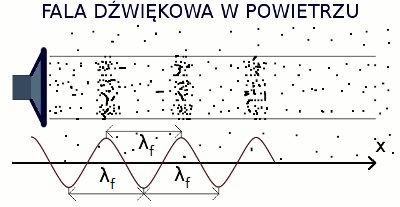
\includegraphics[width=10cm]{Zdjecia/2/fala_podluzna}
\caption{Przykład fali podłużnej}
\label{fig:fala_podluzna}
\end{figure}

Długością fali \( \lambda_f \) nazywamy odległoś między dwoma maksimami (lub minimami), które oznaczają maksymalne zagęszczenie (rozrzedzenie) cząstek w materiale.

\subsection{Fale poprzeczne}

Fale poprzeczne propagują w kierunku prostopadłum do kierunku drgań cząstek. Przykładami takich fal są fale elektromagnetyczne, fale propagacji naprężeń w materiale stałym, czy fala na zamocowanym jednostronnie sznurze, pokazana na Rys.2.2. Prędkoś fali poprzecznej w nieograniczonym ośrodku wyraża się wzorem:

\begin{equation}
c_T=\sqrt{\frac{\mu}{\rho}}
\end{equation}
gdzie
\begin{eqwhere}[2cm]
        \item[$c_T$] prędkość fali poprzecznej
        \item[$\mu$] stała Lam\'{e}go
        \item[$\rho$] gęstość ośrodka
\end{eqwhere}

\begin{figure}[h]
\centering
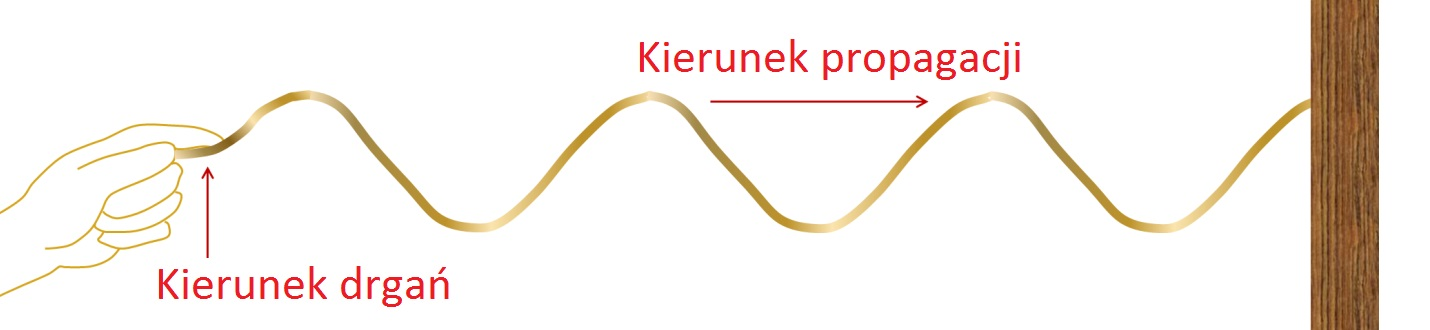
\includegraphics[width=10cm]{Zdjecia/2/fala_poprzeczna}
\caption{Przykład fali poprzecznej}
\label{fig:fala_poprzeczna}
\end{figure}

\subsection{Fale Rayleigha i L\"{o}va}

Opisane wcześniej fale propagują w nieograniczonych mediach. Fale Rayleigha oraz L\"{o}va są falami propagującymi w obszarze powierzchni ciał stałych. Dla fal Rayleigha drgania cząstek odbywają się równolegle oraz prostopadle do kierunku rozchodzenia się fali, zataczając elipsy. Kierunek prostopadły jest normalny do płaszczyzny, na której fala propaguje. Prędkoś fal Rayleigha dla metalu można wyrazić za pomocą współczynnik Poissona i prędkości fal poprzecznych:

\begin{equation}
c_R=\frac{0.87+1.12\cdot\nu}{1+\nu}\cdot c_T
\end{equation}
gdzie
\begin{eqwhere}[2cm]
        \item[$c_R$] prędkość fali Rayleigha
        \item[$c_T$] prędkość fali poprzecznej
        \item[$\nu$] współczynnik Poissona
\end{eqwhere}

Fale L\"{o}va to fale, w których drgania zachodzą w kierunku prostopadłym do kierunku, ale równolegle do płaszczyzny propagacji. Takie fale są wykorzystywane przy badaniu układów wielowarstwowych. Są silnie dyspersyjne, co oznacza że ich prędkość jest funkcją częstotliwości.

\begin{figure}[h]
        \centering
        \begin{subfigure}{0.35\textwidth}
                \centering
	     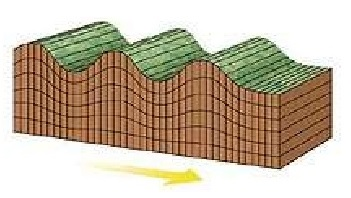
\includegraphics[width=5cm]{Zdjecia/2/fala_rayleigha}
                \subcaption{\label{subfigure_a}}
        \end{subfigure}
        \begin{subfigure}{0.35\textwidth}
                \centering
	     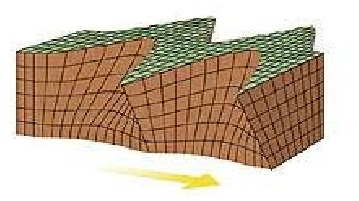
\includegraphics[width=5cm]{Zdjecia/2/fala_lova}
                \subcaption{\label{subfigure_b}}
        \end{subfigure}
        \label{fig:subcaption_example}
        \caption{Fale powierzchniowe: \protect\subref{subfigure_a} fala Rayleigha, \protect\subref{subfigure_b} fala L\"{o}va}
\end{figure}

\subsection{Fale Lamba}

Ważnym typem fal, z racji na szerokie zastosowanie, są fale Lamba. Propagują one na cienkościennych elementach jak płyty, czy rury. Tego typu fale powstają na skutek złożenia dwóch fal Rayleigha, propagujących na płaszczyznach po obu stronach obiektu. Fale Lamba można podzielić na fale symetryczne, kiedy obie fale składowe propagują w tej samej fazie i asntysymetryczne kiedy propagują w innych fazach. Prędkość fal Lamba zależna jest od częstotliwości, ze względu na dyspersyjny charakter.

\begin{figure}[h]
\centering
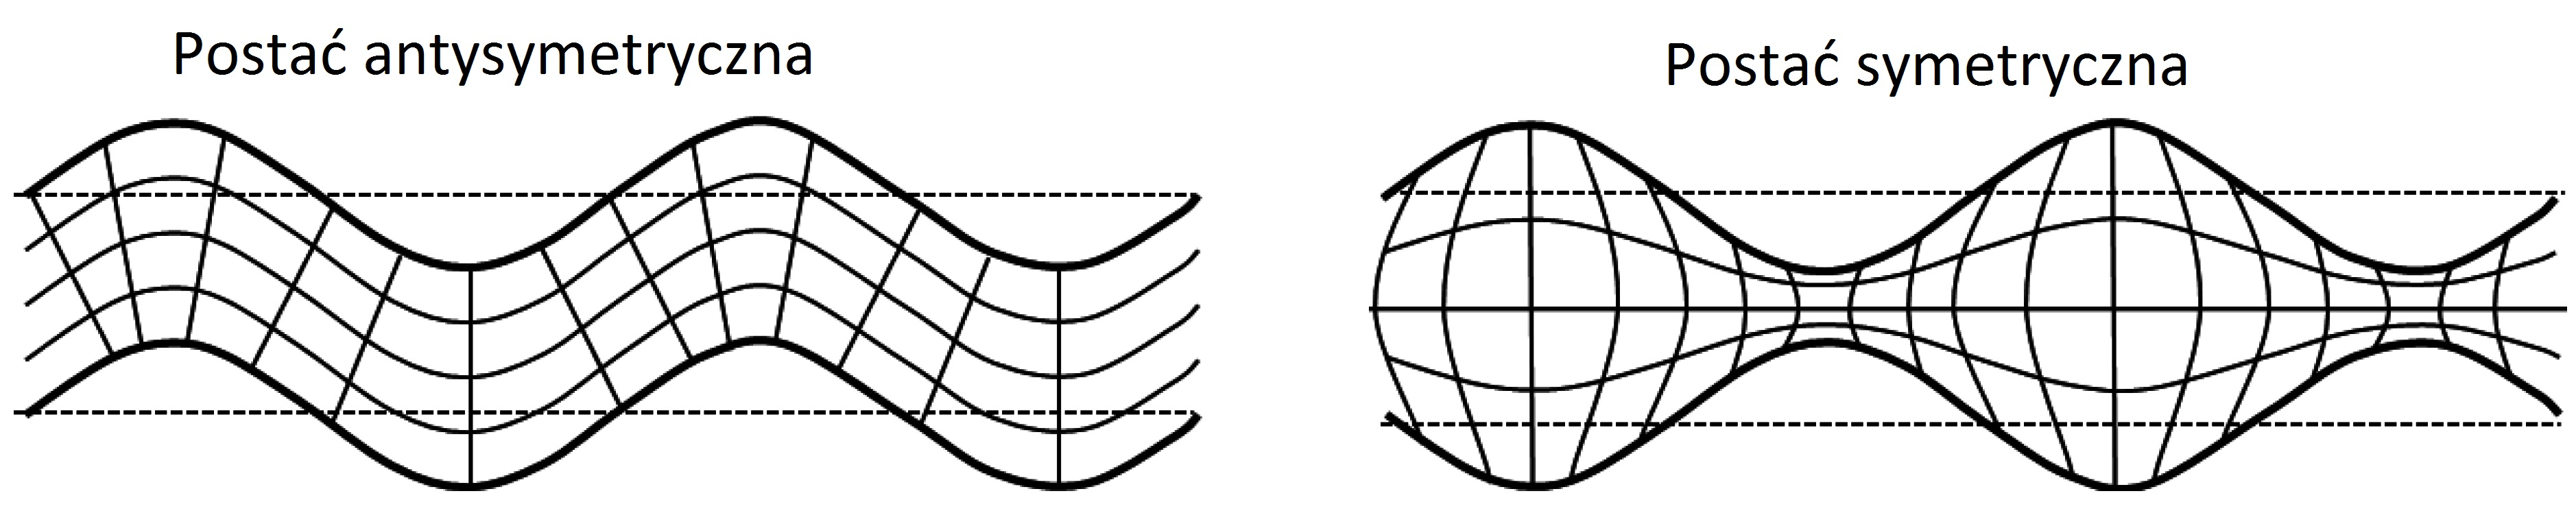
\includegraphics[width=14cm]{Zdjecia/2/fala_lamba}
\caption{Fale Lamba}
\label{fig:fala_lamba}
\end{figure}

%---------------------------------------------------------------------------
























\section{Zjawisko dyspersji}
\label{sec:rodzaje_fal_sprezystych}

Dyspersja jest zjawiskiem zależności prędkości propagacji fali od jej częstotliwości. Częstotliwością fali nazywamy liczbę pełnych przebiegów (np. od maximum do maximum) w jednostce czasu. Jednostką częstotliwości jest herc (Hz). Wielkością równie często używaną jest częstość kołowa dana wzorem \( \omega = 2\pi f \). Jej jednostką jest radian na sekundę [rad/s]. Odpowiednikiem tego parametru dla wymiarów geometrycznych jest liczba falowa. Określa ona jak wiele długości fali zawiera fala w jednostce odległości. Jednostką liczby falowej jest radian na metr [rad/m].

\begin{figure}[h]
\centering
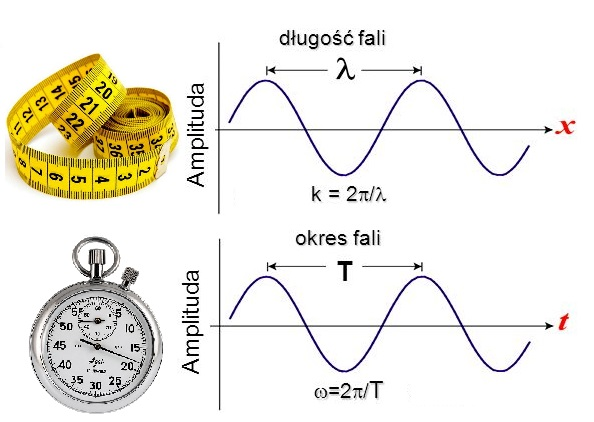
\includegraphics[width=10cm]{Zdjecia/2/czestotliwosc1}
\caption{Częstotliwość \( \omega \) i liczba falowa k}
\label{fig:czestotliwosc_i_liczba_falowa}
\end{figure}


Kiedy mówimy o krzywych dyspersji, możemy mieć na myśli zależności liczby falowej od częstotliwości, prędkości fazowej od częstotliwości lub prędkości grupowej od częstotliwości. Na rysunku \ref{fig:krzywe_k_od_omega} znajdują się przykładowe charakterystyki k(\(\omega\)) postaci fal Lamba dla aluminiowej płyty o grubości 1mm.

\begin{figure}[h]
\centering
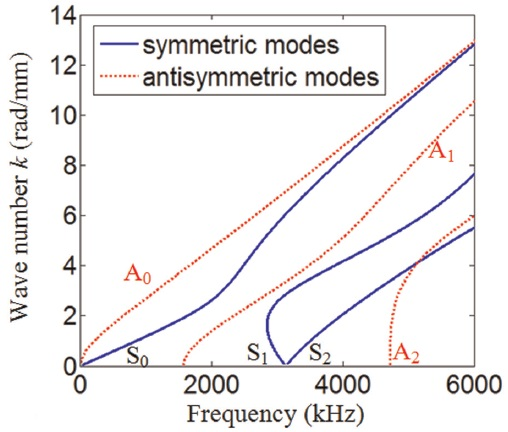
\includegraphics[width=10cm]{Zdjecia/2/char_fazowa}
\caption{Krzywe k(\(\omega\)) \cite{bartek_tian}}
\label{fig:krzywe_k_od_omega}
\end{figure}

Na wykresach widać jedną rzecz, ważną dla zastosowań fal prowadzonych - są one multimodalne. Z wykresów wynika, że w najkorzystniejszym do analizy przypadku propagują dwa mody, jeden symetryczny i jeden antysymetryczny. Wraz ze wzrostem częstotliwości propagującej fali pojawiają się dodatkowe jej postaci, co znacznie utrudnia analizę danych z przebiegów. Jednym ze sposobów ograniczania liczby modów, jest wprowadzanie wymuszeń o niskich częstotliwościach.

\subsection{Prędkość fazowa i grupowa}

Prędkość fazowa określa jak szybko przemieszcza się punkt fali o stałej fazie. Dla fali sinusoidalnej u(x,t)=sin(kx-\(\omega\)t) można wyznaczyć zależność na prędkość fazową w następujący sposób:

\begin{equation}
kx-\omega t=const \Rightarrow \frac{d(kx-\omega t)}{dt}=0 \Rightarrow k\frac{dx}{dt}-\omega=0
 \Rightarrow \frac{dx}{dt}=\frac{\omega}{k}
\end{equation}

Jak widać dla skończonej wartości \(\omega\) i k dążącego do zera, prędkość fazowa rośnie do nieskończoności. Dla przypadku pierwszych modów, gdzie zarówno k jak i \(\omega\) zmierzają do zera, sytuacja wygląda różnie. Na rysunku \ref{fig:krzywe_vp_od_omega} znajduje się przykładowy wykres zależności prędkości fazowej od iloczynu częstotliwości i grubości materiału dla cienkościennej rury. W przypadku fal prowadzonych dla elementów cienkościennych, często wykreśla się charakterystyki z zaznaczeniem wpływu grubości ściany. Na wykresie widać, że wszystkie mody poza pierwszymi dwoma dążą prawostronnie do nieskończoności. Pozostałe dwa zachowują się odmiennie - jeden wykres dąży do 0 (postać antysymetryczna), a drugi do wartości skończonej (postać symetryczna).

\begin{figure}[h]
\centering
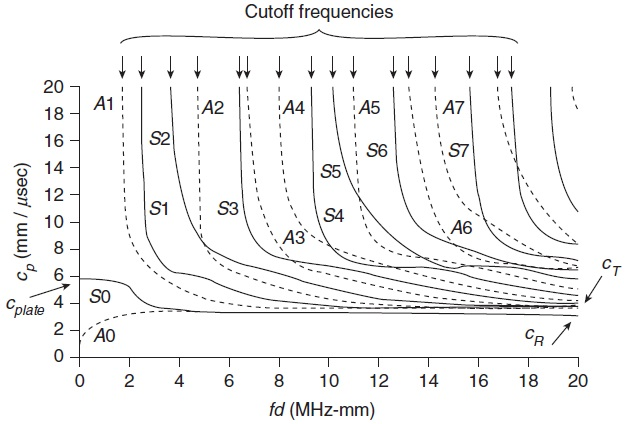
\includegraphics[width=10cm]{Zdjecia/2/char_predkosc_fazowa}
\caption{Krzywe \(V_p(\omega\)) \cite{bartek_rose}}
\label{fig:krzywe_vp_od_omega}
\end{figure}

Jeśli fala składa się z więcej niż jednej składowej sinusoidalnej, które mają różne prędkości, należy określić jeszcze prędkość grupową.  Prędkość każdej z pojedynczych składowych, będzie jej prędkością fazową. Prędkość grupowa dotyczy sygnału, złożonego ze wszystkich składowych. Można ją prezentować jako prędkość punktu o zmiennej fazie na wykresie sygnału, np. maximum, jak na rysunku \ref{fig:przykladowy_sygnal}.

\begin{figure}[h]
\centering
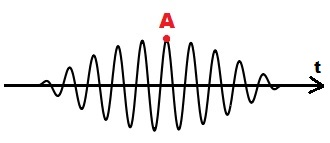
\includegraphics[width=10cm]{Zdjecia/2/predkosc_grupowa_wierzcholek}
\caption{Przykładowy sygnał. Prędkość punktu A jest prędkością grupową}
\label{fig:przykladowy_sygnal}
\end{figure}

Weźmy sygnał złożony z kilku sinusoid o zbliżonej częstości. Fazę każdego sygnału można zapisać jako \( \omega_i t - k_i T + \phi_i \), gdzie \( i\) oznacza numer składowej. Założmy, że fazy tych sygnałów są równe w punkcie x=0, t=0. Wynika stąd, że \( \phi_i \) są niezależne od \( \omega \). Punkt x=0, t=0 będzie maksimum, ponieważ wszystkie składowe zsumują się w tym punkcie. Aby znaleźć kolejny punkt z takim maximum, należy określić gdzie fazy po raz kolejny będą sobie równe.  Punkt, w którym to zjawisko zajdzie musi być niezależny od \( \omega \), w otoczeniu pewnego \( \omega \). Symbolicznie można to zapisać jako:

\begin{equation}
\frac{d(\omega t - kx - \phi)}{d\omega}=0 \Rightarrow t-\frac{dk}{d\omega}x=0 \Rightarrow \frac{x}{t}=\frac{d\omega}{dk}
\end{equation}

Maximum sygnału będzie więc w każdym punkcie x, t spełniającym powyższą zależność. Prędkość grupowa fali jest więc równa:

\begin{equation}
V_g=\frac{dw}{dk}
\end{equation}

Z samego faktu istnienia takiej zależności nie wynika, że w sygnale znajdzie się jakiś charakterystyczny punkt, propagujący z taką prędkością. Wynika z niej natomiast, że jeśli takowy punkt będzie, to będzie się poruszał z prędkością grupową. Należy jeszcze wspomnieć o wyznaczaniu prędkości grupowej sygnału o składowch, o różnych wartościach \( \omega \). W takim przypadku należy prędkość grupową wyznaczyć dla wartości \(\omega\) sygnału dominującego. Dominujący sygnał można znaleźć przy pomocy przekształecenia Fouriera.

Na rysunku \ref{fig:predkosc_grupow_wykres} znajdują się przykładowe krzywe, przedstawiające prędkość grupową dla fal Lamba, dla cienkościennej płyty aluminiowej.

\begin{figure}[h]
\centering
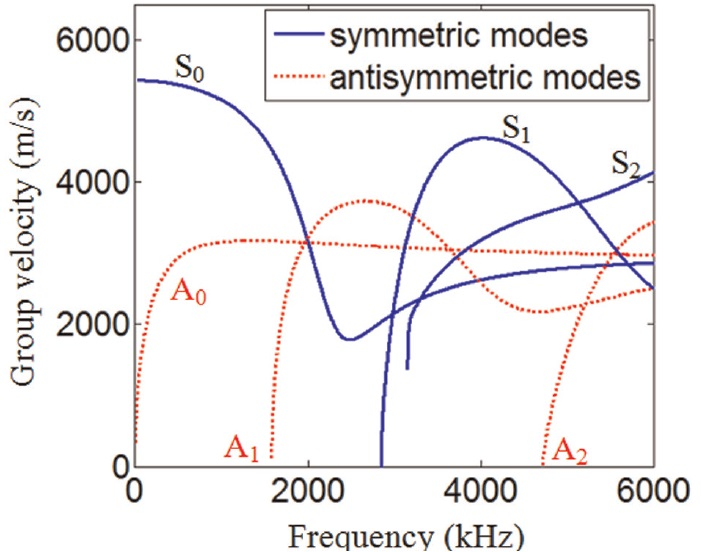
\includegraphics[width=10cm]{Zdjecia/2/predkosc_grupowa_wykres}
\caption{Wykres prędkości grupowej \(V_g(\omega)\) \cite{bartek_tian}}
\label{fig:predkosc_grupow_wykres}
\end{figure}


\subsection{Analityczne wyznaczanie krzywych dyspersji}

Zależności dyspersyjne są trudne, a często niemożliwe do wyznaczenia w sposób analityczny. Dla prostych przypadków rozwiązania analityczne są znane, a kilka z nich jest poniżej opisanych w celu lepszego wyjaśnienia zjawiska dyspersji.
Pierwszym przypadkiem będzie model nieskończenie długiej, napiętej sprężyny, przedstawionej na rysunku \ref{fig:nieskonczenie_krotki_odcinek_sprezyny}.

\begin{figure}[h]
\centering
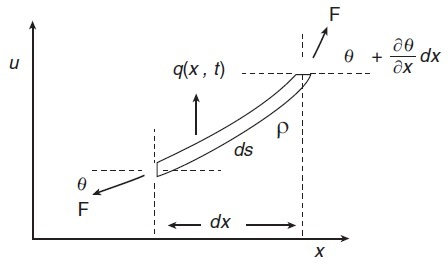
\includegraphics[width=10cm]{Zdjecia/2/dyspersja_analitycznie_sprezyna}
\caption{Nieskończenie krótki odcinek napiętej sprężyny \cite{bartek_rose}}
\label{fig:nieskonczenie_krotki_odcinek_sprezyny}
\end{figure}

Symbole z rysunku oznaczają:

\begin{eqwhere}[2cm]
        \item[$ds$] długość sprężyny
        \item[$\theta$] kąt przyłożenia siły zewnętrznej
        \item[$F$] siły wewnętrzne
        \item[$q$] siła oddziaływania sprężyny na jednostkę długości ugięcia
        \item[$\rho$] masa sprężyny na jednostkę długości.
\end{eqwhere}

Korzystając z drugiej zasady dynamiki Newtona, zapisujemy równanie ruchu układu:

\begin{equation}
-Fsin\theta+Fsin(\theta+\frac{\partial \theta}{\partial x}dx)+qds = \rho ds \frac{\partial^2u}{\partial t^2}.
\end{equation}

Załóżmy dodatkowo, że:

\begin{equation}
ds \approx dx\; ,\; sin\theta=\theta \; i\; \theta = \frac{\partial u}{\partial x}.
\end{equation}

To pozwala uprościć równanie:

\begin{equation}
-F\theta+F(\theta + \frac{\partial \theta}{\partial x}dx)=\rho dx\frac{\partial^2 u}{\partial^2 t}
\end{equation}

\begin{equation}
F\frac{\partial^2 u}{\partial x^2} + q = \rho \frac{\partial^2 u}{\partial^2 t}.
\end{equation}

Jeśli założymy brak siły zewnętrznej, to otrzymujemy proste równanie falowe:

\begin{equation}
\frac{\partial^2 u}{\partial x^2} = \frac{1}{c_0^2} \frac{\partial^2 u}{\partial^2 t},\quad c_0=\sqrt{\frac{F}{\rho}}
\end{equation}

gdzie
\begin{eqwhere}[2cm]
        \item[$c_0$] prędkość fali.
\end{eqwhere}

Przyjmijmy rozwiązanie w postaci:

\begin{equation}
u(x,t)=Ae^{i(kx-\omega t)}.
\end{equation}

Jeśli wstawimy je do równania falowego to otrzymamy zależność dyspersyjną:

\begin{equation}
\omega^2=c_0^2 k^2.
\end{equation}

Jest to przypadek liniowej zależności \( k(\omega)\), a więc dyspersja fali nie zachodzi. W takim przypadku prędkość fazowa, jest równa prędkości grupowej:

\begin{equation}
V_p=\frac{\omega}{k}=\frac{d\omega}{dk}=V_g
\end{equation}

Prosta modyfikacja układu ze sprężyną jak na rysunku \ref{fig:nieskonczenie_krotki_odcinek_sprezyny2}, powoduje skomplikowanie zależności dyspersyjnej.

\begin{figure}[h]
\centering
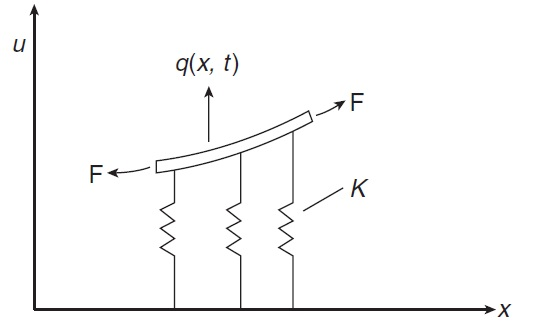
\includegraphics[width=10cm]{Zdjecia/2/dyspersja_analitycznie_sprezyna2}
\caption{Nieskończenie krótki odcinek napiętej sprężyny na sprężystym podłożu \cite{bartek_rose}}
\label{fig:nieskonczenie_krotki_odcinek_sprezyny2}
\end{figure}

Przyjmijmy siłę \(q=-Ku(x,t)\), co prowadzi do równania równowagi:

\begin{equation}
\frac{\partial^2 u}{\partial x^2} - \frac{K}{F}u = \frac{1}{c_0^2} \frac{\partial^2 u}{\partial^2 t}.
\end{equation}

Ponownie załóżmy rozwiązanie w postaci \( u(x,t)=Ae^{i(kx-\omega t)} \) i podstawmy je do równania równowagi. Prowadzi to do zależności:

\begin{equation}
\Big(-k^2-\frac{K}{F}+\frac{w^2}{c_0^2}\Big)e^{i(kx-\omega t)}=0.
\end{equation}

Równanie to jest nazywane równaniem charaktersytycznym (lub dyspersyjnym). Rozwiązaniem jest:

\begin{equation}
-k^2-\frac{K}{F}+\frac{w^2}{c_0^2}=0.
\end{equation}

Zależność \(k(\omega)\) przyjmuje postać:

\begin{equation}
k^2=\frac{w^2}{c_0^2}-\frac{K}{F}.
\end{equation}

Podstawiając \( k=\frac{\omega}{c_p}\), otrzymujemy :

\begin{equation}
c_p = \sqrt{c_0^2\Bigg( \frac{1}{1 - \frac{c_0^2 K}{\omega^2 F} } \Bigg)}.
\end{equation}

Jak widać w takim przypadku prędkość fazowa jest zależna od częstotliwości, a więc będzie zachodzić dyspersja fali.

\vspace{3mm}

Kolejnym problemem wartym wspomnienia, jest problem propagacji fal Lamba w cienkiej, nieskończonej płycie. Płyta wraz z przyjętym układem współrzędnych znajduje się na rysunku \ref{fig:nieskonczona_plyta}.

\begin{figure}[h]
\centering
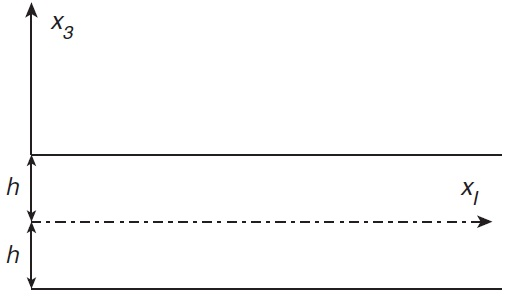
\includegraphics[width=10cm]{Zdjecia/2/dyspersja_analitycznie_plyta}
\caption{Nieskończona płyta \cite{bartek_rose}}
\label{fig:nieskonczona_plyta}
\end{figure}

Jest kilka metod rozwiązania takiego zagadnienia, ale nie są opisane one w tej pracy (metoda potencjałów, metoda fal cząstkowych). Jeśli przyjmiemy zerowe naprężenia na płaszczyznach zewnętrznych jako warunki początkowe, to związki dyspersyjne przyjmują zależności:

\begin{equation}\label{fig:RL1}
\frac{tan(qh)}{tan(ph)}=-\frac{4k^2pq}{(q^2-k^2)^2}
\end{equation}
dla postaci symetryczych oraz

\begin{equation}\label{fig:RL2}
\frac{tan(qh)}{tan(ph)}=-\frac{(q^2-k^2)^2}{4k^2pq}
\end{equation}
dla postaci antysymetrycznych,

gdzie
\begin{equation}
p^2=\frac{\omega^2}{c_L^2} - k^2 \; ,a \; q^2=\frac{\omega^2}{c_L^2}-k^2
\end{equation}

\begin{eqwhere}[2cm]
        \item[$c_T$] prędkość fali poprzecznej
	\item[$c_L$] prędkość fali podłużnej
\end{eqwhere}

Równania \ref{fig:RL1}, \ref{fig:RL2} nazywają się równaniami Rayleigha-Lamba i są nierozwiązywalne w sposób analityczny. Jest to przykład bardziej skomplikowanego modelu, gdzie możliwe jest wyznaczenie związków \(k\) i \(\omega\), ale do wykreślenia krzywych dyspersji konieczne jest zastosowanie metod numerycznych.



\subsection{Numeryczne wyznaczanie krzywych dyspresji}
Pierwszym przypadkiem numerycznego wyznaczania krzywych dyspersji, jest rozwiązanie równań Rayleigha-Lamba przedstawionych w poprzedniej sekcji. Zakładamy, że interesują nas tylko rozwiązania rzeczywiste, które pojawią się jeśli k przyjmie wartości rzeczywiste bądź urojone (w równaniach występuje tylko czynnik \(k^2\)).

Poniżej znajdują się równania Rayleigha-Lamba w postaci ułatwiającej proponowany sposób rozwiązania:

\begin{equation}
\frac{tan(qh)}{q}+\frac{4k^2ptan(ph)}{{q^2-k^2}^2}=0
\end{equation}

\begin{equation}
qtan(qh)+\frac{{(q^2-k^2)}^2tan(ph)}{2k^2p}=0.
\end{equation}

\vspace{5mm}

Rozwiązać równanie możemy według przedstawionego algorytmu.

\begin{enumerate}
  \item Wybierz iloczyn \((\omega h)_0\).
  \item Wybierz początkową estymatę prędkości fazowe \((c_p)_0\) (a pośrednio też \(k\)).
  \item Oblicz znak lewych stron równań R-L.
  \item Wybierz kolejną wartość prędkości fazowej \((c_p)_1 > (c_p)_0\) i policz znaki lewych stron jeszcze raz.
  \item Powtarzaj kroki 3 i 4 aż znaki się zmienią. Oznaczać to bedzie, że pierwiastek równania znajduje się pomiędzy ostatnio wybranymi prędkościami. Załóżmy, że jest to pomiędzy \( (c_p)_n \) i \( (c_p)_{n+1} \).
  \item Wykorzystaj jakiś algorytm iteraycjny do znalezienia pierwiastka \(c_p\) z odpowiednią dokładnością.
   \item Po znalezienu pierwiastka, kontynuuj wyszukiwnie kolejnych pierwiastków dla założonego \( (\omega h)_0 \), powtarzając kroki 2-6.
  \item Wybierz kolejną wartość \( \omega h \) i wykonaj dla niej kroki 2-7.
\end{enumerate}

\vspace{5mm}

W ten sposób łatwo wyznaczyć krzywe dyspersji, ale należy zaznaczyć, że równania dyspersyjne zostały obliczone analitycznie dla konkretnego przypadku struktury, jaką jest płyta. Metody numeryczne ograniczają się w tym przypadku do rozwiązania wyznaczonych równań. Możliwość ogólniejszego podejścia do badań numerycznych, dla szerokiego wachlarza struktur daje metoda elementów skończonych.

Metoda ta daje możliwości dokładnego przewidzenia odpowiedzi dynamicznych, dla złożonych układów mechanicznych. Jeśli założymy przypadek małych odkształceń, to problem można zapisać w postaci równania różniczkowego:

\begin{equation} \label{eq:MES1}
M\ddot u + Ku = f^{ext}
\end{equation}

gdzie
\begin{eqwhere}[2cm]
        \item[$M$] macierz mas układu
        \item[$K$] macierz sztywności układu 
        \item[$u$] przemieszczenia punktów układu
        \item[$f^{ext}$] wektor sił zewnętrznych
\end{eqwhere}

Sposobem wyznaczenia krzywych dyspersji z tak określonego układu, może być rozwiązanie równania tj. znalezienie pola przemieszczeń dla wszystkich węzłów w dyskretnych chwilach czasowych, a następnie obliczenie wielowymiarowego przekształcenia Fouriera otrzymanego sygnału.

Równanie można rozwiązać na przykład z wykorzystaniem centralnej formuły różnicowej dla \( \ddot u\):

\begin{equation}
\ddot x = \frac{u^{t+1} - 2u^t + u^{t-1}}{\Delta t^2}.
\end{equation}

Po podstawienu otrzymujemy zależność:

\begin{equation}
\frac{1}{\Delta t^2}M(u^{t-1}-2u^t+u^{t-1}) + Ku^t = f^t
\end{equation}

\begin{equation}
u^{t+1}=\Delta t^2 M^{-1}(f^t -Ku^t)+2u^t-u^{t-1}
\end{equation}

gdzie \( t \) oznacza obecną chwilę czasową, a \( t+1 \) chwilę kolejną.
Operacja odwracania macierzy mas jest kosztowna obliczeniowo. Można przyśpieszyć obliczenia przez zastosowanie skupionej macierzy mas (wyrazy niezerowe tylko na głownej diagonali).

Jeśli interesuje nas propagacja tylko w jednym kierunku, to dla obliczonego sygnału \( u[m, n] \) (m - liczba kroków czasowych \(\Delta t \) , n - liczba kroków geometrycznych \(\Delta x\) w kierunku x) przekształcenie Fouriera można obliczyć według wzoru:

\begin{equation} \label{eq:fourier_2d}
U[p, q] = \sum_{k=0}^{m-1} \sum_{l=0}^{n-1} u[k, l]e^{-i2\pi (-p \frac{k}{m} + q\frac{l}{n})}
\end{equation}

Mając dyskretną postać przekształcenia Fouriera można wykreślić krzywe dyspersji, wyznaczając dla każdej próbki wartość czętotliwości i liczby falowej. Można to zrobić wiedząc, że częstość zawiera się w przedziale \([0, \frac{1}{2\Delta t}2\pi]\), a liczba falowa \([0, \frac{1}{2\Delta x}2\pi]\). Przykładowe krzywe przedstawione są na rysunku \ref{fig:krzywe_dyspersji_tian1}.

\vspace{5mm}

\begin{figure}[h]
\centering
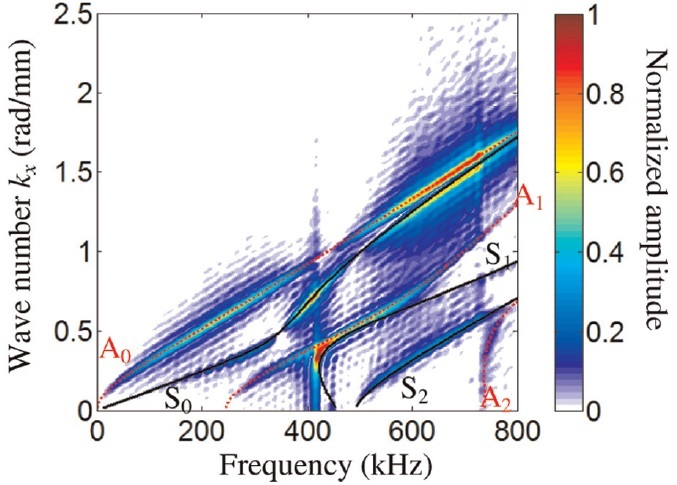
\includegraphics[width=10cm]{Zdjecia/2/dyspersja_tian1}
\caption{Krzywe dyspersji wyznaczone przy pomocy dwuwymiarowego DFT}
\label{fig:krzywe_dyspersji_tian1}
\end{figure}

Innym sposobem wyznaczania krzywych dyspersji z pomocą modelu MES, jest symulacja układu dla wymuszeń harmonicznych o ustalonych częstotliwościach, w których chcemu wyznaczyć krzywe. Jako przyład rozpatrzmy jednorodny pręt. Dla przypadku pręta wymuszanego na jednej płaszczyźnie przekroju, dane należy zebrać przed odbiciem fali od swobodnego końca pręta, tak aby sygnał propagował tylko w jednym kierunku. W liniach równoległych do osi, obliczamy pola prędkości przemieszczenia punktów. Może to być też pole przemieszczeń lub naprężeń, ale pole prędkości jest stosunkowo łatwe do wyznaczenia.
Znając już prędkości dla wszystkich punktów w jednej lini, w chwili t, możemy wyznaczyć widmo otrzymanego sygnału. Następnie z widma sygnału odczytujemy liczby falowe, dla których powstały widoczne piki. Pik dla największej liczby falowej dotyczy pierwszego modu, a każdy kolejny, z coraz mniejszymi liczbami falowymi, modów kolejnych.

Pole prędkości można wyznaczyć na podstawie różnycowych formuł centralnych \ref{eq:MES2} oraz \ref{eq:MES3}.

\begin{equation} \label{eq:MES2}
\dot u^{t+1} = \dot u^n + \frac{\Delta t}{2}(\ddot u^n + \ddot u^{n+1})
\end{equation}

\begin{equation} \label{eq:MES3}
u^{n+1} = u^n + \Delta t(\dot u^n + \frac{\Delta t}{2}\ddot u^n)
\end{equation}

Załóżmy, że znamy pełne rozwiązanie w chwili t. Przemieszczenie w chwili t+1 możemy więc obliczyć z zależności \ref{eq:MES3}. Następnie podstawiamy wynik do równania \ref{eq:MES1} i obliczamy przyspeszenie w chwili t+1. Ostatecznie korzystając z formuły \ref{eq:MES2} możemy wyznaczyć prędkość w chwili t+1.

Przykładowe widmo, z którego możemy odczytać liczby falowe czterech modów znajduje się na rysnuku \ref{fig:widmo_wymuszenie1}. Jak widać nie wszystkie liczby falowe da się wykryć przy pomocy danych z jednej lini, więc niezbędne jest prowadzenie obliczeń dla kilku różnych linii.

\begin{figure}[h]
\centering
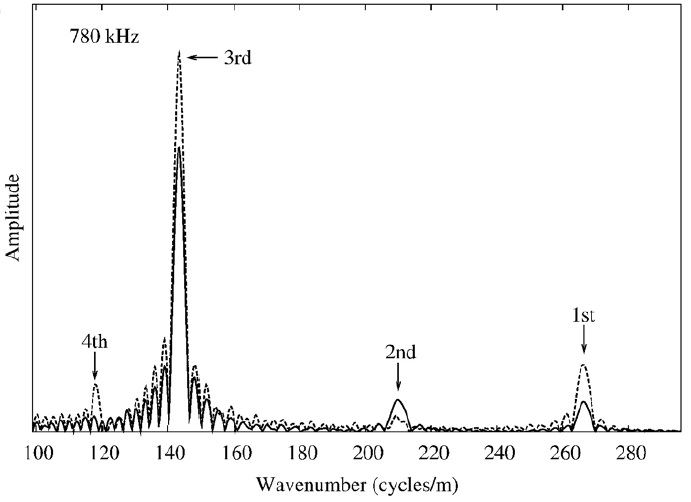
\includegraphics[width=10cm]{Zdjecia/2/widmo_wymuszenia_waskopasmowe}
\caption{Widmo sygnału prędkości na liniach równoległych do osi pręta}
\label{fig:widmo_wymuszenie1}
\end{figure}

Wadą tego sposobu jest konieczność prowadzenia obliczeń dla każdej częstotliwości, dla jakiej chcemy mieć punkty krzywych dyspersji. Jedne przebieg daję nam tylko jeden punkt na każdej krzywej. Fakt prowadzenia obliczeń tylko w liniach równoległych do osi pręta, ogranicza dodatkow obszar propagujących fal do fal podłużnych.

\vspace{3mm}

Sposobem zmniejszenia liczby symulacji jakie trzeba przeprowadzić jest symulacja z wymuszeniem szerokopasmowym. Pozwala to na uzyskanie informacji o krzywych dyspersji, dla częstotliwości zawierających się w wymuszającym sygnale. Pojawia się jednak kilka dodatkowych kroków jakie trzeba wykonać, aby uzyskać liczby falowe modów dla poszczególnych częstotliwości.

Aby uzyskać dane do wykreślenia krzywych dyspersji, należy obliczyć przestrzenny rozkład prędkości na liniach równoległych do osi dla wszystkich częstotliwości. W tym celu trzeba wykonać następujące czynności.

\begin{enumerate}
  \item Wyznaczyć odpowiedzi czasowe dla każdego punktu na interesującej nas lini równoległej do osi pręta.
  \item Obliczyć transformaty Fouriera tych sygnałów
  \item Z widma sygnału w każdym punkcie pobrać informacje o amplitudzie dla kolejnych częstotliwości. Na tej podstawie odtworzyć amplitudowy przebieg sygnału na całej lini dla każdej interesującej nas częstotliwości.
  \item Dla obliczonych w pkt. 3 przebiegów, obliczyć transformatę Fouriera i z wykresu odczytać wartości liczby falowej, dla wybranych częstotliwości.
\end{enumerate}

Rysunki \ref{fig:szer_odp_czasowe} oraz \ref{fig:szer_odp_przestrzenne} przedstawiają kolejne kroki postępowania, dla odpowiedzi na wymuszenie krokiem jednostkowym preta zbudowanego z 1601 węzłów na długości jednej lini. 

\begin{figure}[h]
\centering
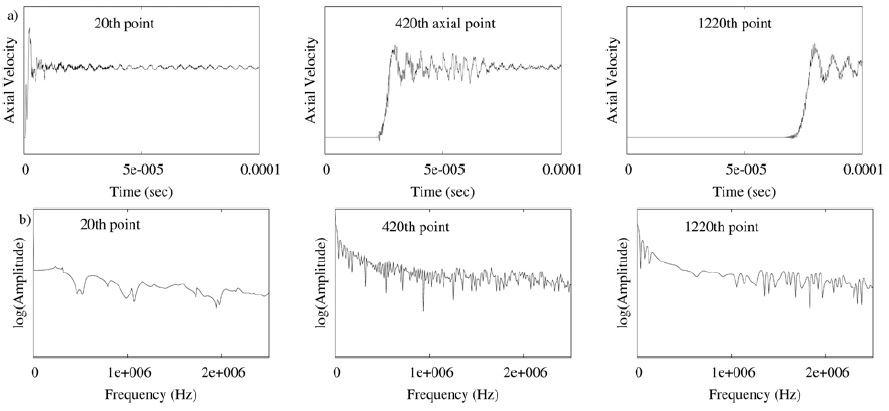
\includegraphics[width=12cm]{Zdjecia/2/widmo_wymuszenia_szerokopasmowe1}
\caption{a) Odpowiedzi na szerokopasmowe wymuszenie w wybranych punktach jednej lini b) Przekształcenia Fouriera odpowiedzi czasowych}
\label{fig:szer_odp_czasowe}
\end{figure}

\begin{figure}[h]
\centering
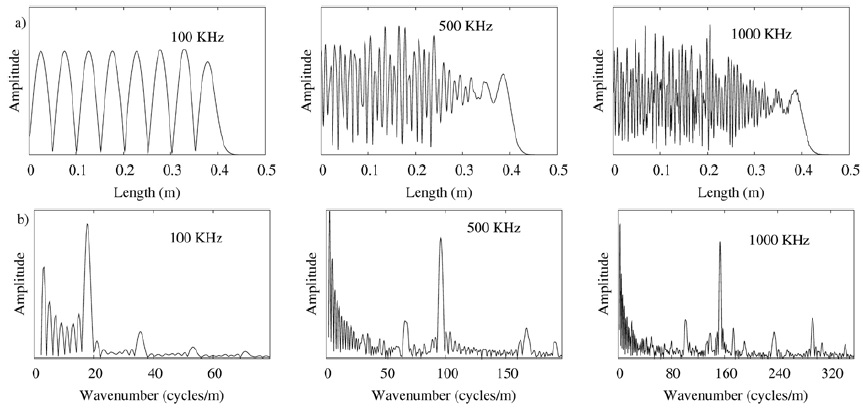
\includegraphics[width=12cm]{Zdjecia/2/widmo_wymuszenia_szerokopasmowe2}
\caption{a) Odtworzony sygnał apmlitudowy na długości pręta w jednej lini b) Przekształcenie Fouriera odtworzonych sygnałów}
\label{fig:szer_odp_przestrzenne}
\end{figure}

\vspace{3mm}

Ostatnia przedstawiona tutaj metoda skupia się, na rozwiązaniu zagadnienia własnego modelu wyznaczonego z pomocą MES. Tym razem zakładać będziemy wybraną liczbę falową i dla niej obliczać częstości poszczególnych modów. 
Po raz kolejny za przykład weźmy pręt. Pręt dzielimy na komórki, które będą się składać z kolejnych płaszczyzn, na których znajdują się węzły. Znając odległość płaszczyzn i wybierając liczbę falową, możemy okrelić przesunięcie fazowe fali pomiędzy płaszczyznami. Sytuacja przedstawiona jest na rysunku \ref{fig:komorki_preta}.


\begin{figure}[h]
\centering
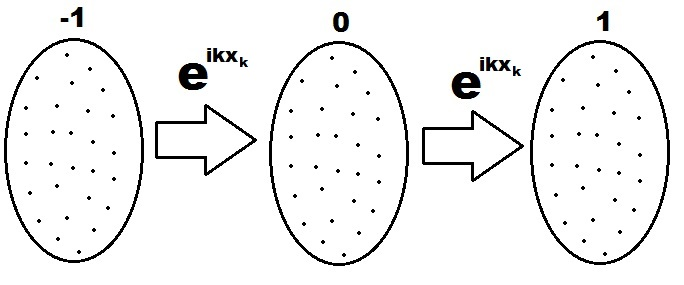
\includegraphics[width=10cm]{Zdjecia/2/metoda_numeryczna3}
\caption{Kolejne komórki pręta}
\label{fig:komorki_preta}
\end{figure}

W liniowych systemach do opisu popagacji fali wystarcza jedna komórka i siły wewnętrzne pochodzące od komórek sąsiednich. W przypadku braku sił zewnętrznych i przy założeniu skupionej macierzy mas, równanie układu można zapisać w postaci \ref{eq:MES4}. Rysunek \ref{fig:komorki_preta_sztywnosc} przedstawia sposób wyznaczania macierzy sztywności dla komórki środkowej, z uwzględnieniem zależności z komórkami sąsiednimi.

\begin{equation} \label{eq:MES4}
M_0\ddot x_0 + \sum_{p=-1}^1 K_p x_p = 0
\end{equation}

\begin{figure}[h]
\centering
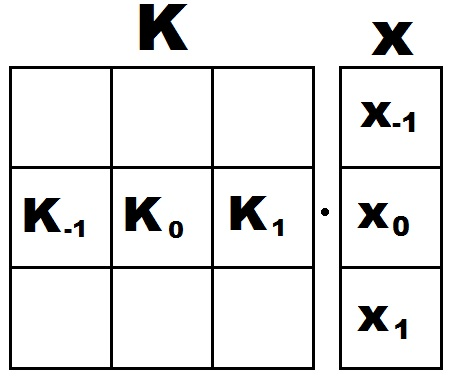
\includegraphics[width=8cm]{Zdjecia/2/metoda_numeryczna3_sztywnosc}
\caption{Wyznaczanie macierzy sztywności środkowej komórki z uwzględnieniem zależności z komórkami sąsiednimi}
\label{fig:komorki_preta_sztywnosc}
\end{figure}

Uwzględniając wszystkie informacje równanie układu można zapisać jako \ref{eq:MES5}. Podstawiając dodatkowo zależności \( \ddot x = x \omega^2 \), \( M_{sys} = M_0 \) oraz \( K_{sys} = K_{-1} e^{-ikx_k} + K_0 + K_1 e^{ikx_k} \) otrzymujemy równanie \ref{eq:MES6}.

\begin{equation} \label{eq:MES5}
M_0\ddot x_0 + K_{-1} x_0 e^{-ikx_k} + K_0 x_0 + K_1 x_0 e^{ikx_k} = 0
\end{equation}

\begin{equation} \label{eq:MES6}
 (M_{sys}\omega^2 + K_{sys})x_0 = 0
\end{equation}

Ostatecznie rozwiązując zagadnienie własne dla pary macierzy \( M_{sys} \) i \( K_{sys} \) otrzymujemy kwadraty częstości własnych układu dla założonego \( k \). Każda z częstości należy do jednego modu krzywych dyspersji.

Wadami tej metody są konieczność prowadzenia obliczeń dla każdej liczby falowej, którą chcemy uwzględnić w wynikach, oraz brak dokładnej informacji, która częstość własna należy do której postaci fali.

Dużą zaletą z kolei jest fakt, że wyznaczamy jedną metodą krzywe dyspersji dla fal podłużnych i poprzecznych.

Przykładowe krzywe dyspersji uzyskane w ten sposób przedstawia rysunek \ref{fig:przykladowe_krzywe}.

\begin{figure}[h]
\centering
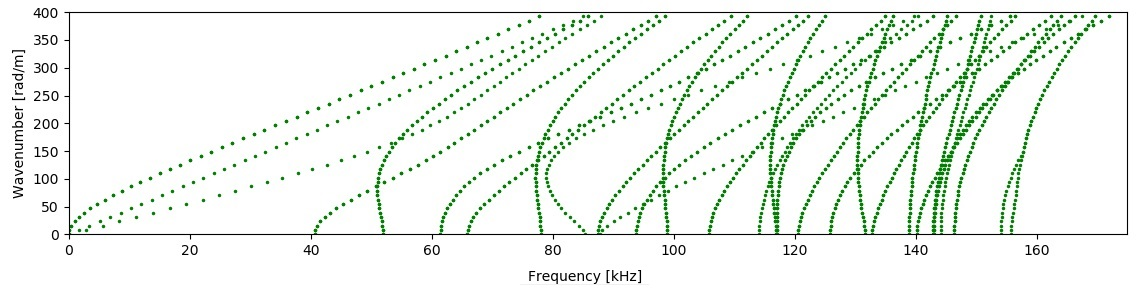
\includegraphics[width=14cm]{Zdjecia/2/przykladowe_krzywe}
\caption{Krzywe uzyskane przez wielokrotne rozwiązanie zagadnienia własnego pręta}
\label{fig:przykladowe_krzywe}
\end{figure}



\subsection{Eksperymentalne wyznaczanie krzywych dyspersji}

Eksperymentalne badania fal prowadzonych przeprowadza się wzbudzając odpowiednio obiekt, a następnie zbiera się dane o powstałej fali w innych punktach konstrukcji lub w tym samym punkcie po odbiciu fali. Zebrane dane analizuje się za pomocą algorytmów, w których duże znaczenie ma przekształcenie Fouriera.

Jako wzbudniki fal prowadzonych często stosowane są przetworniki piezoelektryczne (na przykład z ceramik PZT). Proste zjawisko piezoelektryczne z jakiego korzystają takie przetworniki, pozwala przekształcić energię elektryczną na energię mechaniczną. Efekt odwrotny pozwala zbierać informację o energi odkształcenia w materiale i sygnał mechaniczny przekształcić w elektryczny. 

Materiały piezoelektryczne znalazły szerokie zastosowanie ze względu na dobre parametry mechaniczne, odporność na wiele substancji chemicznych oraz bardzo duże możliwości kształtowania przetworników. Wzbudniki i sensory piezoelektryczne często występują jako cienkie fragmenty materiału piezoelektrycznego, które można wykonać w dowolnym kształcie. W przypadku kiedy chcemy uzyskać większą apmlitudę wzbudzenia, stosuje się stosy stworzone z wielu warstw piezoelektryka.

Obecna ilość dostępnych na rynku rozwiązań pozwala na dobranie odpowiedniego przetwornika do niemal każdego projektu bazującego na niskich częstotliwościach. Podczas analizy rozwiązań komercyjnych okazało się, że duża część takich przetowrników posiada ograniczenia działania do kilku kHz. Jest to najczęściej zbyt niska częstotliwość, nawet w przypadku badania wyłącznie modów podstawowych. Dostępne są też rozwiązania dla częstotliwości do nawet kilkuset kHz, co w przypadku fal prowadzonych może stanowić wystarczającą wartość.

Przykłady przetworników piezoelektrycznych w formie płytki oraz stosu znajdują się na rysunku \ref{fig:piezoelektryki}.

\begin{figure}[h]
        \centering
        \begin{subfigure}{0.35\textwidth}
                \centering
	     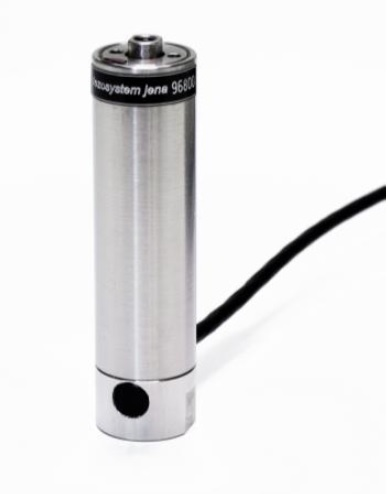
\includegraphics[width=5cm]{Zdjecia/2/piezo_stos}
                \subcaption{\label{subfigure_a}}
        \end{subfigure}
        \begin{subfigure}{0.35\textwidth}
                \centering
	     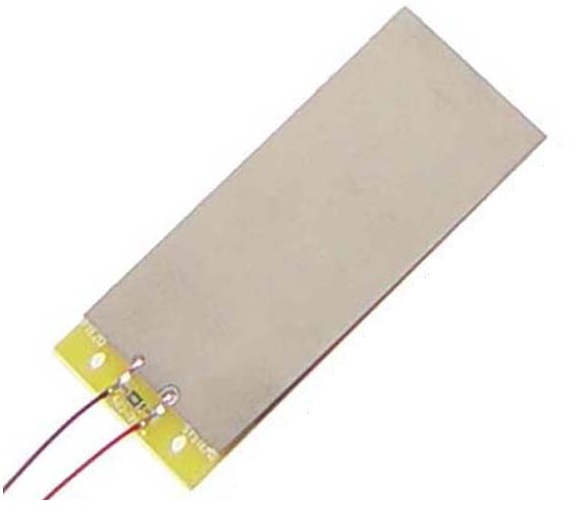
\includegraphics[width=5cm]{Zdjecia/2/piezo_plytka}
                \subcaption{\label{subfigure_b}}
        \end{subfigure}
        \caption{Przetworniki piezoelektryczne: \protect\subref{subfigure_a} w formie sotsu, \protect\subref{subfigure_b} w formie płytki}
        \label{fig:piezoelektryki}
\end{figure}

\vspace{3mm}

Innym sposobem badań jest wykorzystanie techniki laserowej. Za pomocą wiązki lasera możliwe jest wzbudzenie fal sprężystych w materiale. Na szczególną uwagę zasługuje możliwość wzbudzenia fali krótki impulsem, którego widmo będzie miało bardzo duży zakres częstotliwości. Sygnał taki możemy porównać do delty Diraca, dla której widmo ma stałą amplitudę. 

Za pomocą lasera możemy wykonywać także pomiary drgań materiału. Posłużyć może do tego na przykład interferometr laserowy, wykorzystujący efekt Dopplera. Detekcja jest jednak ograniczona do fal powierzchniowych. Atutem takiego pomiaru jest możliwość wykonania go dla wielu punktów na badanym obiekcie. Dzięki temu możemy uzyskać przestrzenny obraz propagacji fali.

Przykładowe stanowisko do badania płyt za pomocą wymuszenia laserem przedstawia rysunek \ref{fig:laser}.

\begin{figure}[h]
\centering
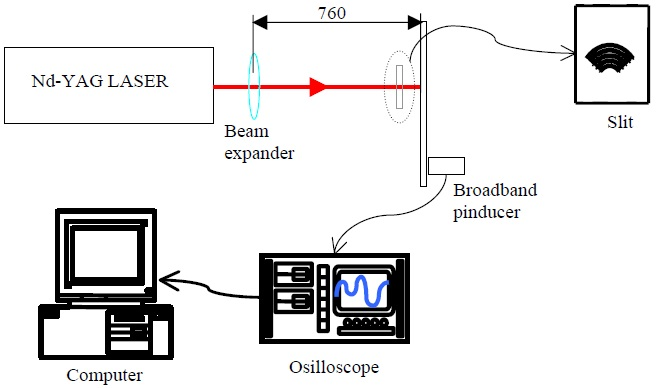
\includegraphics[width=10cm]{Zdjecia/2/laser}
\caption{Przykładowy układ stanowiska do badania fal Lamba w cienkiej płycie \cite{bartek_tian}}
\label{fig:laser}
\end{figure}


%Wzbudzalnosc w sekcji dyspersja

\subsection{Wyznaczanie krzywych wzbudzalności}

Krzywe wzbudzalności określają zależność amplitudy od częstotliwości fali dla poszczególnych jej modów i dla danego wymuszenia. Dla pewnych przypadków można wyznaczyć taką zależność analitycznie, jednak podobnie jak w przypadku krzywych dyspersji, nie jest to metoda uniwersalna. Poniżej znajdują się wyłącznie przykładu numerycznych sposobów wyznaczania tego typu krzywych, ponieważ mają one szersze zastosowanie.

Pierwszy sposób wykorzystuję standardowy model MES ze wzoru \ref{eq:MES1}. Wyznaczamy przemieszczenia węzłów w pewnych chwilach czasowych , a następnie obliczamy wielowymiarowe przekształcenie Fouriera na zgromadzonych danych \ref{eq:fourier_2d}. Wynikiem transformacji jest zależność częstości i liczby falowej, co pozwala wykreślać krzywe dyspersji, a dodatkowo trzecia oś, prostopadła do pozostałych, zawiera informacje o amplitudzie. Przedstawiając na płaszczyźnie zależność amplitudy od liczby falowej, otrzymamy krzywe wzbudzalności.

\vspace{3mm}

Innym sposobem omawianym w literaturze jest zastosowanie metody SAFE (Semi-Analytical Finite Element). Jest ona modyfikacją metody elementów skończonych, polegającą na ustaleniu analitycznego rozwiązania problemu, dla jednego kierunku propagacji. W przypadku problemu trójwymiarowego pozwala to na tworzenie elementów dwuwymiarowych, w kierunkach propagacji, dla których nie znamy rozwiązania. Dzięki temu cały model jest prostszy i szybszy w rozwiązaniu. Sformułowanie takie jest jednak złożone i nie będzie tutaj przytaczane w całości. Jest ono opisane dokładniej w \cite{bartek_fabien}.

Wynikiem wykorzystania metody SAFE jest związek siły wymuszającej i przemieszczenia węzłów modelu. Związek ten przedstawia wzór \ref{eq:wzbudzanie1}. Wzbudzalność określić można na podstawie macierzy E. Określa ona dla modu m, związek pomiędzy siłą przyłożoną w i-tym węźle i przemieszczeniu j-tego węzła \( (\textbf{E}_m)_{ij} \). Rysunek \ref{fig:wzbudzalnosc1} przedstawia wzbudzalność obliczoną dla pierwszych dwóch modów w dwuwarstwowej płycie, bez tłumienia.

\begin{equation} \label{eq:wzbudzanie1}
\textbf{U} = \sum_{m=1}^M \textbf{E}_m \textbf{F}(k_m) e^{ik_m z}
\end{equation}

gdzie
\begin{eqwhere}[2cm]
	\item[$U$] wektor przemieszczenia węzłów
	\item[$E$] macierz wzbudzalności
	\item[$U$] siła wymuszająca w dziedzinie liczby falowej
	\item[$z$] kierunek propagacji, dla którego założono rozwiązanie analityczne
	\item[$m$] numer modu
	\item[$M$] liczba propagujących modów
	\item[$k$] liczba falowa dla m-tego modu.	
\end{eqwhere}

\begin{figure}[h]
\centering
\includegraphics[width=10cm]{Zdjecia/2/wzbudzalnosc1}
\caption{Krzywe wzbudzalności dla dwuwarstwowej cienkiej płyty \cite{bartek_fabien}}
\label{fig:wzbudzalnosc1}
\end{figure}

Kolejna metoda polega na porównaniu prac modów dla fal Lamba z tzw. modem wirtualnym . Prowadzi ona do zależności na wzbudzalność dla cienkich płyt:

\begin{equation} \label{eq:wzbudzanie2}
a_m =  \textbf{X}_m^{(b), H} \frac{\textbf{F}(z)}{i\textbf{P}_{(a:m),(b)}}.
\end{equation}

gdzie

%\begin{equation} \label{eq:wzbudzanie2}
%P_{(a:m),(b)} = \textbf{X}_m^{(b), H} (\textbf{K}_{+1}^{(b),H} e^{-k^{(b)}\Delta x} - \textbf{K}_{-1}^{(b),H} e^{+ik^{(b)}\Delta x} - \textbf{K}_{+1}^{(a)} e^{+ik_m^{(a)}\Delta x} + \textbf{K}_{-1}^{(a)} e^{-ik_m^{(a)}\Delta x})\textbf{X}_{0,m}^{(a)} = 0
%\end{equation}

\begin{equation} \label{eq:wzbudzanie3}
\textbf{P}_{(a:m),(b)} = \textbf{X}_m^{H} (\textbf{K}_{+1}^{H} e^{-ik\Delta x} - \textbf{K}_{-1}^{H} e^{+ik\Delta x} - \textbf{K}_{+1} e^{+ik\Delta x} + \textbf{K}_{-1} e^{-ik\Delta x})\textbf{X}_{0}
\end{equation}

\begin{eqwhere}[2cm]
	\item[$a_m$] amplituda m-tego modu w odpowiedzi na wymuszenie
	\item[$\textbf{F}(z)$] siła wymuszająca działająca wzdłuż grubości płyty
	\item[$\textbf{X}$] wektory własne 
	\item[$\textbf{K}_{\pm 1}$] macierz sztywności dla kolejnej/poprzedniej płaszczyzny propagacji
	\item[$k$] liczba falowa
	\item[$x$] kierunek propagacji
	\item[$m$] numer modu	
	\item[$a_m$] mod numer m, dla pola falowego a
	\item[$b$] mod wirtualny b	
	\item[$H$] sprzężenie hermitowskie.
\end{eqwhere}

Należy zaznaczyć, że do obliczenia amplitud poszczególnych modów, konieczna jest znajomość krzywych dyspersji (zależności \( k(\omega) \) ), oraz wektorów własnych odpowiadających częstościom własnym, dla których wyznaczamy amplitudy.

\subsection{System sing\_around (lub Self-Excited Acoustical System)}

Systemy sing-around to samowzbudne systemy, do pomiaru parametrów rezonansowych fal. Idea systemu polega na dodatnim sprzężeniu zwrotnym pomiędzy przetwornikiem pomiarowym oraz wzbudnikiem. Badanie konstrukcji rozpoczyna arbitralny sygnał wzbudzający. Przetwornik pomiarowy odbiera sygnał i przetwarza go na sygnał elektryczny, który jest odpowiednio filtrowany i wzmacniany, a następnie podawany do wzbudnika. Dane pomiarowe są przesyłane do systemu akwizycji i obróbki, w celu wydobycia informacji o stanie konstrukcji. Schemat przykładowego stanowiska badawczego znajduje się na rysunku \ref{fig:sing_around}.

\begin{figure}[h]
\centering
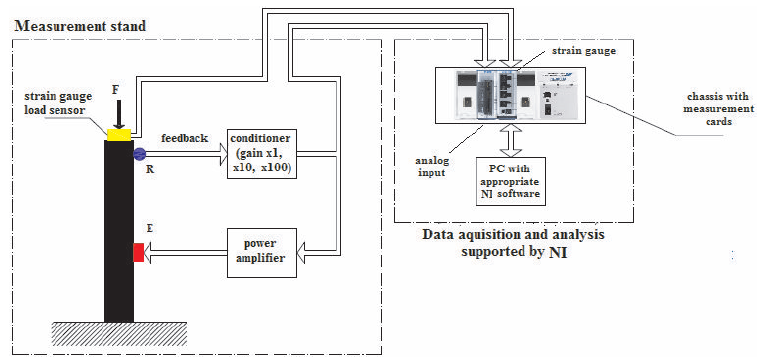
\includegraphics[width=10cm]{Zdjecia/2/sing_around}
\caption{Stanowisko badawcze z systemem sing around \cite{bartek_kwach}}
\label{fig:sing_around}
\end{figure}

Popularnym zastosowaniem tego typu systemów jest pośredni pomiar naprężeń, które mają związek z częstotliwością rezonansową układu bądź prędkością fali, które zmieniają się wraz z odkształcaniem się materiału. Praktycznym przykładem jest pomiar częstotliwości rezonansowej słupa podporowego silosa cementu. Na rysunkach \ref{fig:sing_around_silos} i \ref{fig:sing_around_wyniki} znajduje się widok stanowiska pomiarowego oraz wyniki pomiarów, dla zwiększania i zmniejszania się masy cementu w silosie. W ciągu minuty do silosa dostarczane jest 500kg cementu (125 kg na podporę), a jedno rozładowanie to ok. 2500kg (625 kg na podporę). Przedstawione wyniki dotyczą konfiguracji E1, R1, gdzie E1 to wzbudnik, a R1 to przetwornik pomiarowy.

\begin{figure}[h]
\centering
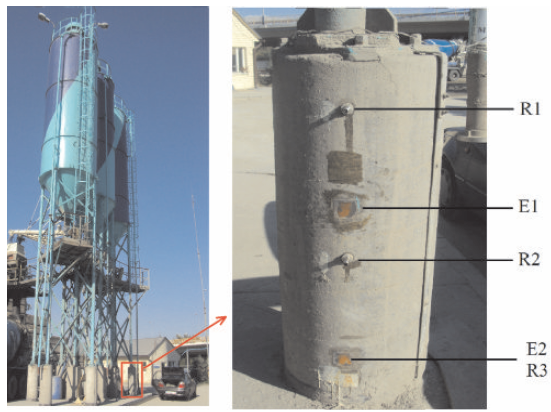
\includegraphics[width=10cm]{Zdjecia/2/sing_around_silos}
\caption{Widok podpory silosa z zamontowanymi przyżadami \cite{bartek_kwach}}
\label{fig:sing_around_silos}
\end{figure}

\begin{figure}[h]
\centering
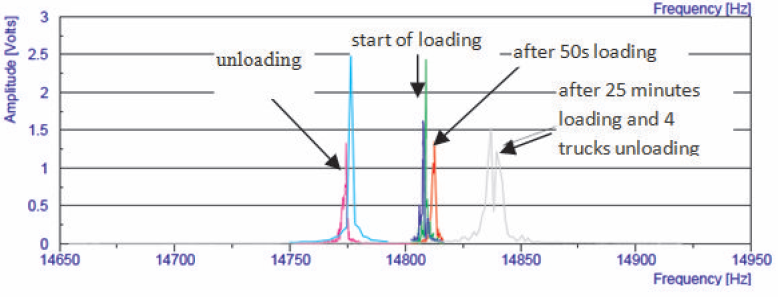
\includegraphics[width=14cm]{Zdjecia/2/sing_around_wyniki}
\caption{Wyniki pomiaru dla ciągłego dostarczania cementu do silosa \cite{bartek_kwach}}
\label{fig:sing_around_wyniki}
\end{figure}

Jak widać częstotliwość rezonansowa zwiększa się wraz ze wzrostem naprężeń ściskających w badanej podporze. Tego typu systemy mają ogromne możliwości zastosowań w różnego typu konstrukcjach, gdzie istotne jest monitorowanie naprężeń.

Znajomość krzywych dyspersji oraz krzywych wzbudzalności dla określonego wymuszenia pozwala zasymulować działanie układu sing-around. Sygnał wyjściowy dla symulacji przebiegu fali, należy podać jako wejście do kolejnej symulacji. Uwzględnienie krzywych dyspersji pozwala określić sposób pomiaru, dla sygnału, który rozbiega się w czasie. Krzywe wzbudzalności pozwalają wyznaczyć piki rezonansowe w widmie badanego sygnału.


%---------------------------------------------------------------------------






















%---------------------------------------------------------------------------



















